\documentclass[letterpaper,12pt,oneside]{article}
\usepackage[utf8]{inputenc}
\usepackage{graphicx}

\usepackage[left=0.3in, right=1in, bottom=0.4in, top=0in]{geometry}

\usepackage[dvipsnames]{xcolor}
\definecolor{orange}{RGB}{127,127,160}

\usepackage{hyperref}
\hypersetup{colorlinks,urlcolor=orange}
\usepackage{setspace}
\usepackage{newtxtext}
\usepackage{array}
\usepackage[export]{adjustbox}
\usepackage[document]{ragged2e}
\renewcommand{\labelitemi}{$\diamond$}
\pagenumbering{gobble}
\begin{document}
    \begin{tabular}{m{4.2in} m{2.5in}}
        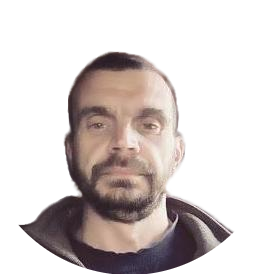
\includegraphics[width=1.8in,left]{photo.png} &
        \vspace{1in}

        \begin{flushright}
        {
        \Huge{Paolo Veronelli}  
        \noindent\rule{2.5in}{0.2pt}
        \begin{normalsize}
        \href{https://github.com/paolino}{github.com/paolino}  
        \href{mailto:paolo.veronelli@gmail.com}{paolo.veronelli@gmail.com}
        \end{normalsize}
        }
        \end{flushright}
        \end{tabular}
    \section*{Education}
        \begin{itemize}
            \item High School, 1984-1989.
            \item Ontology and applied semantics for resource scheduling, 2002-2004 
            \item Utrecht Summer School for Applied Functional Programming , 2016
            \item Functional programming principles (\href{https://www.coursera.org/account/accomplishments/certificate/8NVXL4Y3XUB6}{certificate}) (Scala), 2016
            \item Functional programming design (\href{https://www.coursera.org/account/accomplishments/certificate/WTU8B8G54N79}{certificate}) (Scala), 2016
            \item Parallel Programming (\href{https://www.coursera.org/account/accomplishments/certificate/YU7BSRL8VFTT}{certificate}) (Scala), 2017
        \end{itemize}
    \section*{Works}
        \begin{itemize}
            \item Resource scheduling application for mechanical industry (Python), 2000-2001 
            \item Geometry and energetic numerical approximations for a parabolic lamp mirror    (Python), 2001-2002 
            \item RDF based CMS \href{http://pytypus.cvs.sourceforge.net/viewvc/pytypus/}{Pytypus}  (Python) , 2002-2003 
            \item System Administrator at \href{http://tinvention.net}{Tinvention} (FreeBSD, Apache, MySQL, Tomcat) , 2003
            \item AI libraries, SOMA, NN feed-forward, recursive, with reservoir (Python, Haskell), 2004-2010. 
            \item Image pattern recognition, 2004-2006 (Haskell). 
            \item Full stack development of \href {https://lambdasistemi.net/reactivegas}{Reactivegas} (Haskell, SQLite, JS) 2010-2011 
            \item Salesmen shifts planning algorithm, Fidenza Village, Paul Smith shop (Haskell), 2011-2012 
            \item Full stack development of the cashier system for Emporio Solidale, Borgo val di Taro (PHP, SQLite), 2013 
            \item 1D and 2D genetic search algorithms for stock cut of wood and glass (Haskell), 2013-2014 
            \item Self organizing mesh of radio nodes , prototype and simulator (C, Arduino, Haskell) , 2014 
            \item QR driven environmental game for the Festival della Comunicazione (Haskell), 2015 
            \item Persistent structures for sub-linear operations in link-cut trees, a PhD cooperation (prof. Juan Carlos Saenz Carrasco) (Haskell), 2016-now  
            \item Tram-line discrete event simulation (Haskell), 2016 
        \end{itemize}

\end{document}

